% Options for packages loaded elsewhere
\PassOptionsToPackage{unicode}{hyperref}
\PassOptionsToPackage{hyphens}{url}
%
\documentclass[
]{book}
\usepackage{amsmath,amssymb}
\usepackage{lmodern}
\usepackage{ifxetex,ifluatex}
\ifnum 0\ifxetex 1\fi\ifluatex 1\fi=0 % if pdftex
  \usepackage[T1]{fontenc}
  \usepackage[utf8]{inputenc}
  \usepackage{textcomp} % provide euro and other symbols
\else % if luatex or xetex
  \usepackage{unicode-math}
  \defaultfontfeatures{Scale=MatchLowercase}
  \defaultfontfeatures[\rmfamily]{Ligatures=TeX,Scale=1}
\fi
% Use upquote if available, for straight quotes in verbatim environments
\IfFileExists{upquote.sty}{\usepackage{upquote}}{}
\IfFileExists{microtype.sty}{% use microtype if available
  \usepackage[]{microtype}
  \UseMicrotypeSet[protrusion]{basicmath} % disable protrusion for tt fonts
}{}
\makeatletter
\@ifundefined{KOMAClassName}{% if non-KOMA class
  \IfFileExists{parskip.sty}{%
    \usepackage{parskip}
  }{% else
    \setlength{\parindent}{0pt}
    \setlength{\parskip}{6pt plus 2pt minus 1pt}}
}{% if KOMA class
  \KOMAoptions{parskip=half}}
\makeatother
\usepackage{xcolor}
\IfFileExists{xurl.sty}{\usepackage{xurl}}{} % add URL line breaks if available
\IfFileExists{bookmark.sty}{\usepackage{bookmark}}{\usepackage{hyperref}}
\hypersetup{
  pdftitle={Buscatierra},
  pdfauthor={Facundo Grehan},
  hidelinks,
  pdfcreator={LaTeX via pandoc}}
\urlstyle{same} % disable monospaced font for URLs
\usepackage{longtable,booktabs,array}
\usepackage{calc} % for calculating minipage widths
% Correct order of tables after \paragraph or \subparagraph
\usepackage{etoolbox}
\makeatletter
\patchcmd\longtable{\par}{\if@noskipsec\mbox{}\fi\par}{}{}
\makeatother
% Allow footnotes in longtable head/foot
\IfFileExists{footnotehyper.sty}{\usepackage{footnotehyper}}{\usepackage{footnote}}
\makesavenoteenv{longtable}
\usepackage{graphicx}
\makeatletter
\def\maxwidth{\ifdim\Gin@nat@width>\linewidth\linewidth\else\Gin@nat@width\fi}
\def\maxheight{\ifdim\Gin@nat@height>\textheight\textheight\else\Gin@nat@height\fi}
\makeatother
% Scale images if necessary, so that they will not overflow the page
% margins by default, and it is still possible to overwrite the defaults
% using explicit options in \includegraphics[width, height, ...]{}
\setkeys{Gin}{width=\maxwidth,height=\maxheight,keepaspectratio}
% Set default figure placement to htbp
\makeatletter
\def\fps@figure{htbp}
\makeatother
\setlength{\emergencystretch}{3em} % prevent overfull lines
\providecommand{\tightlist}{%
  \setlength{\itemsep}{0pt}\setlength{\parskip}{0pt}}
\setcounter{secnumdepth}{5}
\usepackage{booktabs}
\ifluatex
  \usepackage{selnolig}  % disable illegal ligatures
\fi
\usepackage[]{natbib}
\bibliographystyle{apalike}

\title{Buscatierra}
\author{Facundo Grehan}
\date{Verano de 2022}

\begin{document}
\maketitle

{
\setcounter{tocdepth}{1}
\tableofcontents
}
\hypertarget{section}{%
\chapter*{}\label{section}}
\addcontentsline{toc}{chapter}{}

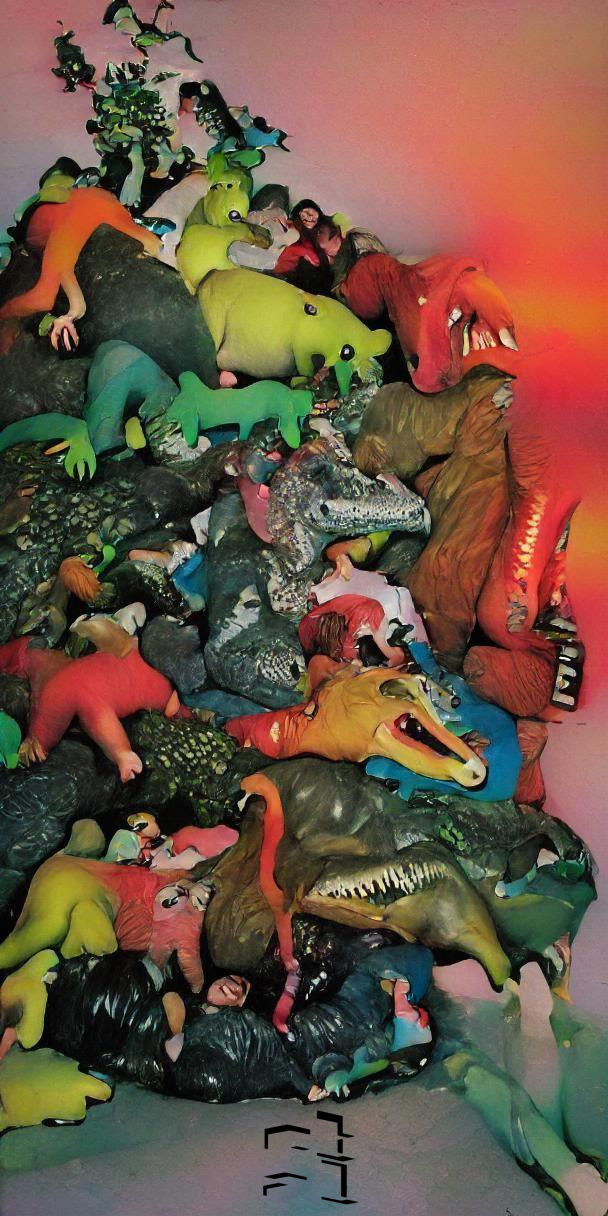
\includegraphics{images/portada.png}

Grehan, Facundo

Buscatierra / 1a ed.~- Ciudad Interdimensional de
Buenos Aires: etal, 2022.

\begin{figure}
\centering
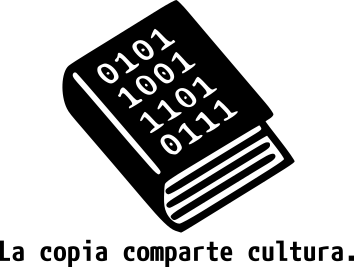
\includegraphics{images/lccc.png}
\caption{🄯2022 - etal. El texto de esta publicación y esta edición se liberan bajo la Licencia de
Producción de Pares}
\end{figure}

\hypertarget{licencia-de-producciuxf3n-de-pares-versiuxf3n-legible-por-humanes}{%
\chapter*{Licencia de Producción de Pares (Versión legible por humanes)}\label{licencia-de-producciuxf3n-de-pares-versiuxf3n-legible-por-humanes}}
\addcontentsline{toc}{chapter}{Licencia de Producción de Pares (Versión legible por humanes)}

\begin{quote}
Esto es un resumen legible por humanos del \href{http://endefensadelsl.org/ppl_es.html}{texto legal (la licencia
completa)}
\end{quote}

\hypertarget{ud.-es-libre-de}{%
\section*{Ud. es libre de}\label{ud.-es-libre-de}}
\addcontentsline{toc}{section}{Ud. es libre de}

\begin{itemize}
\tightlist
\item
  Compartir - copiar, distribuir, ejecutar y comunicar públicamente la obra
\item
  Hacer obras derivadas
\end{itemize}

\hypertarget{bajo-las-condiciones-siguientes}{%
\section*{Bajo las condiciones siguientes:}\label{bajo-las-condiciones-siguientes}}
\addcontentsline{toc}{section}{Bajo las condiciones siguientes:}

\begin{figure}
\centering

\includegraphics{images/by.png}
\caption{\textbf{Atribución} - Debe reconocer los créditos de la obra de la manera
especificada por el autor o el licenciante (pero no de una manera que sugiera
que tiene su apoyo o que apoyan el uso que hace de su obra).}
\end{figure}

\begin{figure}
\centering

\includegraphics{images/sa.png}
\caption{\textbf{Compartir bajo la Misma Licencia} - Si altera o transforma esta obra, o
genera una obra derivada, sólo puede distribuir la obra generada bajo una
licencia idéntica a ésta.}
\end{figure}

\begin{figure}
\centering

\includegraphics{images/nc.png}
\caption{\textbf{No Capitalista} - La explotación comercial de esta obra sólo está permitida
a cooperativas, organizaciones y colectivos sin fines de lucro, a
organizaciones de trabajadores autogestionados, y donde no existan relaciones
de explotación. Todo excedente o plusvalía obtenidos por el ejercicio de los
derechos concedidos por esta Licencia sobre la Obra deben ser distribuidos por y
entre los trabajadores.}
\end{figure}

\hypertarget{entendiendo-que}{%
\section*{Entendiendo que}\label{entendiendo-que}}
\addcontentsline{toc}{section}{Entendiendo que}

\begin{itemize}
\item
  \textbf{Renuncia} - Alguna de estas condiciones puede no aplicarse si se obtiene
  el permiso del titular de los derechos de autor.
\item
  \textbf{Dominio Público} - Cuando la obra o alguno de sus elementos se halle en
  el dominio público según la ley vigente aplicable, esta situación no quedará
  afectada por la licencia.
\item
  \textbf{Otros derechos} - Los derechos siguientes no quedan afectados por
  la licencia de ninguna manera:

  \begin{itemize}
  \item
    Los derechos derivados de usos legítimos u otras limitaciones
    reconocidas por ley no se ven afectados por lo anterior;
  \item
    Los derechos morales del autor;
  \item
    Derechos que pueden ostentar otras personas sobre la propia obra o
    su uso, como por ejemplo derechos de imagen o de privacidad.
  \end{itemize}
\item
  \textbf{Aviso} - Al reutilizar o distribuir la obra, tiene que dejar muy en claro
  los términos de la licencia de esta obra. La mejor forma de hacerlo es
  enlazar a esta página.
\end{itemize}

\hypertarget{lqnh}{%
\chapter{Lo que no hablamos}\label{lqnh}}

otra vez

quedo sola en casa y no sé qué hacer

de aburrida

me someto a un juego de seducción imposible con una piba

hermosa que me cuelga los mensajes pero cuando

me responde me promete

ganas de vernos y sin decirlo una fiesta

biensonante de las pasiones

de amorosa

entusiasmo cariño sin decirlo y mando esos memes esos memes

de apoyo lindo y aguante a seres

que jamás vi en vida

porque de manos largas para querer y confundir

cierto clima con turbios fenómenos de época se trata

tal vez la bola de tejer alianzas entre nosotras

una sensibilidad común

de algún modo

más o menos pero más menos que más

amable

expropiada entre genuinas señales de necesidad y deseo

para mal y para mí

y de borracha pienso mil cosas

que no enrostramos ni afiebradas porque a veces

lo preferible es esta guía de preguntas estudiantiles tan siempre

mal formuladas a la rabia que nos compete y convoca

si por las tardes la tensión ahora es adónde está

el silencio

en dónde la canción

y dónde ese ruidito que pasa por detrás tabanero

como una fauna que no vemos en la especie nuestra que enajena

de su vientre sensible la construcción de un ambiente

propicio para nosotras mi reina

si en la abstracción socializante las penas duran lo que un potro en el tarro

y son gases expandiéndose en el aire para no chocarse

nos queremos

las caritas

con las resolanas frías pero al sol son pan

de muerto la raíz entre el teclado no nos mata ni nos hace más fuertes

más bien muta y lo vuelve a intentar

ojalá que en el futuro seamos como plantas

para crecer de noche y al calor

de la luna hacernos grandes y posibles

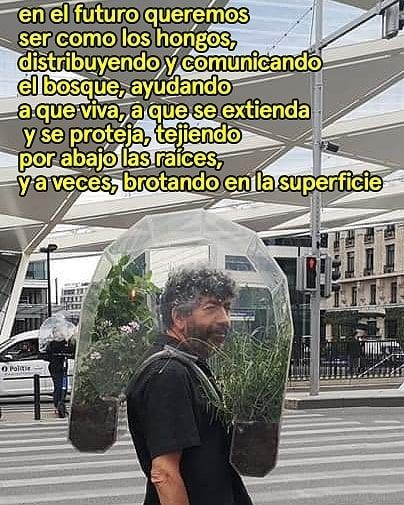
\includegraphics{images/1.png}

nuestras cuerpas las ideas

floreciendo siempre

en lo oscuro

porque a todo esto quise beber del arenal

puse mis músculos en hidroponia

para enredar en nuestros ojos los fantasmas

que en cada suspiro libertamos

y no salvé ni mi lengua del atoro

de este ritual traslaticio madurado en frascos rotos

\hypertarget{meta-verso-y-porqueruxeda}{%
\chapter{Meta verso y porquería}\label{meta-verso-y-porqueruxeda}}

en una charla de académicos sobre memes

a un costado de la ciudad

la alameda del fondo se bate en discursos

no autorizados por el evento un viejo

quizá guerrillero veterano traza el contraste

entre la dominación militar de los 70s

y la dominación tecnológica de este siglo

uno que vino en carreta trayendo

en sus crines un fueguito

a la vereda amiga

interviene y grita que

le deprime te juro me dan ganas de llorar

tanta gente hablando y tanto tiempo de pantallitas

salgan de la televisión manga de

yo estuve internado en dos neuro-

psiquiátricos en esta ciudad el primero

acá cerquita al lado de la cárcel

el segundo era una tumba entre los bordes de la realidad digital

afuera de las redes sociales del estatus y de los likes

pero toda la escena se desviste ahora

en condescendencias inquietas que aplacan las contradicciones del pastito

analógico sobre el que se sostiene la conversa

inexistente de las redes subjetivantes

y los productos culturales que tensionan cada vez más

nuestra senilidad cyborg con nuestros cuerpos

latinoamericanos bola de cringe

frío en la avenida ahora una chica

toca instrumentos caros para cantar

odas al bloqueo gente en internet y me abandono

contentísima a los cauces

de la depresión autolesiva

igual la loca no soy yo porque estetizo dicen

toda una sensibilidad naturalizada por la

neo burguevanguardia glitcheada en tocs

audiencia y sabios entonces escuchan

y simulan bailar en este castillo

que encima dieron por llamar caos o

salud mental o

una revista cultural medio tongocha

para las conciencias privilecarizadas del pero

más tarde cuando otro muchacho ajusta

una guitarra acústica -la vieja viola

el jardín de la casona sufre ahora y de nuevo

el abandono se acrecientan entonces

los yuyos y los flujos

centrífugos de tráfico humano

ya es de noche quizá el músico él sí

un loquito pueda convertirse en lobizón

o de mínima generar de pronto aullidos

anacrónicos que incomoden por de más ciertas

cámaras de eco-

lalia o la estabilidad

simbólica de un mundo enrarecido

que ahora se pierde en esquinas medio zumbantes

de fantasmitas intemporales

y entra sin mucha seguridad pero sí

con un latentísimo agobio medio galopando

a todos los planos de ese infierno que dimos

por llamar circulación de mercancías y reproducción incesante de capital

\hypertarget{rosmeri}{%
\chapter{Rosmeri}\label{rosmeri}}

en las luces verdes tenues del wifi

sobre tus tetas veo

todo el brillo de internet

de tus dibujos y tus memes

a vos chupándome el culo en mi cama en tu casa

acogotando mi grito impudoroso

aun frente a las gatas que aun

cachorras saben la escena como un ritual

de humanas pasiones oyen los claros

trabados en las evocaciones

engalletadas de mi lengua como

un punto medio pero también

como la elipsis

cabeza de ángel

guillotinado para el nuestro sabor

a guiso de nuestros corazones


\includegraphics{images/2.png}

\hypertarget{asuxed-arrulla-la-gata-la-hora}{%
\chapter{Así arrulla la gata la hora}\label{asuxed-arrulla-la-gata-la-hora}}

no desesperes

ante el pavor de estar online sabiendo

que ajustaste tu ansiedad a esta dinámica

y te pervierte

entonces le llamás soledad política

a tu diario de catástrofe

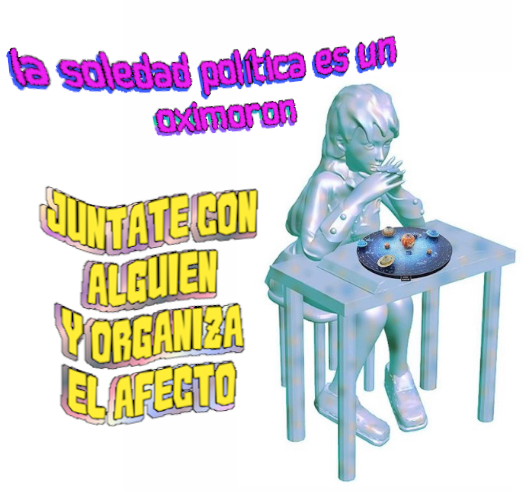
\includegraphics{images/3.png}

no desesperes

\hypertarget{muxfasica-muerta}{%
\chapter{Música muerta}\label{muxfasica-muerta}}

qué de qué ni de cuánto

para alborotar los corazones

a esta utopía roja y helada

dominguera como un cuerno

de feria placera vayamos

a amansar las piedras

cortar un puente intervenir

tres sindicatos

se acaricia y ya digamos

entreverando los albores

de un calor pardo

o veas

y oigas

oigan todas

las cornetas

las fronteras

que atropellamos cual fantasmas

del día que pasó y del mañana que vendrá

a contradecir nuestros hoys

porque este vino me lo guardo

así se me corte y se me pique

otra cumbia otra bartola

se me desconozca

y se reapropie lo apropiado

qué vamos a retener sin el poder

ni cuánto realmente vamos

a conquistar con el transeo

peluches de mediodía cuando miremos

transregida esta calaña

y desmesura articulada

de palabras que no alcanzan

y se

atolondran de pavotas al gallote

campiñero o necrofilia de la dura

no me toques

celebremos

\hypertarget{intenso-antes-de-que-se-me-acaben-los-conjuros}{%
\chapter{Intenso: antes de que se me acaben los conjuros}\label{intenso-antes-de-que-se-me-acaben-los-conjuros}}

soplar soplar soplar

y que el aire exhalado recorra

toda la estepa se cuele entre los acordes de la sierra

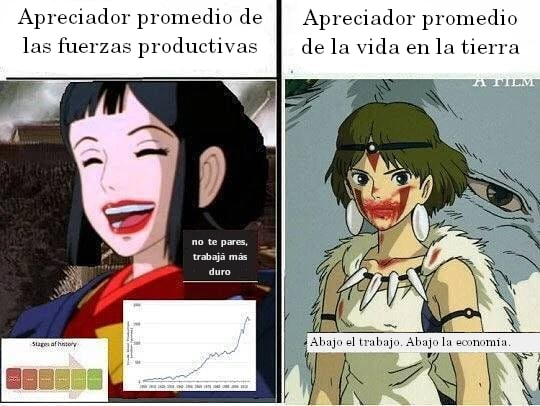
\includegraphics{images/4.png}

lobo de las pasiones compartidas sea mi pecho entero un fuelle

que sople que sople

a un ritmo acompasado pero constante y llegue

mi soplo a la brasa cencerrita

hecho un vendabal de ilusión linda

y le arranque una chispa grande que la convierta en achura viva

\hypertarget{su-paso-un-cuxedrculo-de-ceniza}{%
\chapter{Su paso un círculo de ceniza}\label{su-paso-un-cuxedrculo-de-ceniza}}

ya adivino el ronroneo

de les gatis que al acecho

van marcando mi retorno

del sueño a la vigila pero también

de un clima a otro

lo acomodan a

pura pose larga o fetal casi como dedos

brujos que en el movimiento

surten el conjuro

la necesidad ontológica de convertir la casa

en corazón de batucada silban

y son ellos las que silban podría

decirse franqueando la herida

abierta de la domesticación asilvestrada

porque un gato en cada casa o más

es civilización latente y una toma

del poder se sabe entonces

en su delirio encuentran

siempre a través de otros ojos en cada rostro el rostro del poeta

que por ellos clama sin rescate

perdón señor perdón señora

por mear el árbol de su cora

observan dijimos

observan desde una medianera estrellada algo perdida

el baldío o

la muerte o

la grupa entre los contenedores de la supervivencia quizá el futuro

del afecto carpincho entre nosotras

a contrapelo del psicoanálisis y los desiderativos antropocénicos

porque es otro orden estremecido de pelaje

nunca una mirada bienhabida que consagre las leches de

lo mojado a un malambo

errante por ejemplo

el abejorro

se diría traza

ahora una línea penetrante

en la cancelación

de la existencia estira su extinción y dice mundo

va haber mundo

para siempre

mi vida es efímera y fortuita y al polvo vuelve trascendente

pero los felinos traman incluso hasta

tejen se diría

las olas de la pampa que brotan en una vereda

porque es suya la ciudad en ruinas

y lo saben

la sinfonía agorrionada de los futuros desplomados

sobre sí

mejor dicho devuelven en captura la alianza

interespecies de una comunidad imposible a los trotes mansos de fuerzas que nunca debimos no

y lo sabíamos haber desafiado ay

es otro corte mamífero la peluza transmutada de les gatis

su quejido un codo de amor sublunar y silencioso

no por aspereza pero la rambla conjuga

una manada guerrillera

gatis contra el reino de la mercancía

sino por la anónima utopía

de armar querencia con garritas


\includegraphics{images/5.png}

\hypertarget{salario-precio-y-ganancia}{%
\chapter{salario precio y ganancia}\label{salario-precio-y-ganancia}}

desde que me sacaste esa foto

durmiendo las manos

entre las rodillas y un

almohadón sobre la cara

dejé de preguntarme cuánto hay

de capricho y cuánto de necesidad

en la gestualidad de nuestro comportamiento cotidiano

ahora salgo a pasear un día

de sol las vidrieras

entre mi jornal y el

deseo voy a ellas como endemoniado

para rebotar a fuerza del mantra

estoy contento con el producto que compré y no tengo

que seguir mirando opciones más baratas

estoy contento con el producto

que compré y no tengo

que seguir mirando opciones más baratas

y si hay un interruptor

entre mi intensidad afectiva y

mi modo perro chiquito activado meta

aislamiento concentrado


\includegraphics{images/6.png}

quizá se llame menos masculinidad

frágil en picada que también pero más

autogestión precarizada de la ansiedad

porque hacemos lo que podemos

con lo poco que tenemos

en esta distopía sensible en la que

después millones de años de experiencia humana no

sabemos distinguir

entre el hambre y la sed

entonces cómo ser lindas en un mundo horrible

entonces cómo afectarse para el calor

que o nos convoca

o nos amenaza

\hypertarget{paso-hoy}{%
\chapter{paso hoy}\label{paso-hoy}}

escurrí el trapo de piso y salieron

de él dos almas

en pena. la primera

me dijo que

una característica central del capitalismo avanzado en su estado de descomposición es la incorporación directa de la ciencia al proceso productivo, lo que ha trasformado radicalmente el rol del científico y la misma actividad científica.

la segunda me relojeó:

``¿sos amigo?''

en la iglesia de

la esquina

una plegaria dejé para ellas.

\hypertarget{destajos-de-sensibilidad}{%
\chapter{destajos de sensibilidad}\label{destajos-de-sensibilidad}}

es la hora santa

peluches de mañana

se quedan

en mi cora

para siempre

cuando ellxs marchen sabrán

cargar las armas de esta guerra

(shrek despierta:

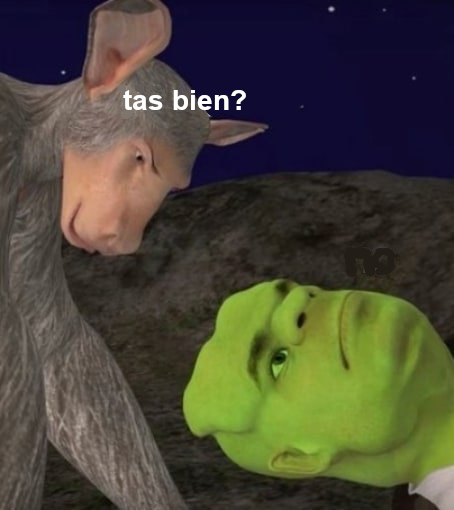
\includegraphics{images/7.png}

somos espíritus afines en la lucha por destituir lo humano

lo euroblanco lo civilizado)

el dembow se empuña como

un calor la cama un boliche

de contaminación

barroca

mestiza

si esta parva de cotorras en orgía

resiste la infiltración de policías

sólo falta lo que falta (viva chile

y lxs que faltan se quedan

para siempre

en nuestro cora

\hypertarget{seruxe1-que-nos-gravita-creciente-la-luna}{%
\chapter{será que nos gravita creciente la luna}\label{seruxe1-que-nos-gravita-creciente-la-luna}}

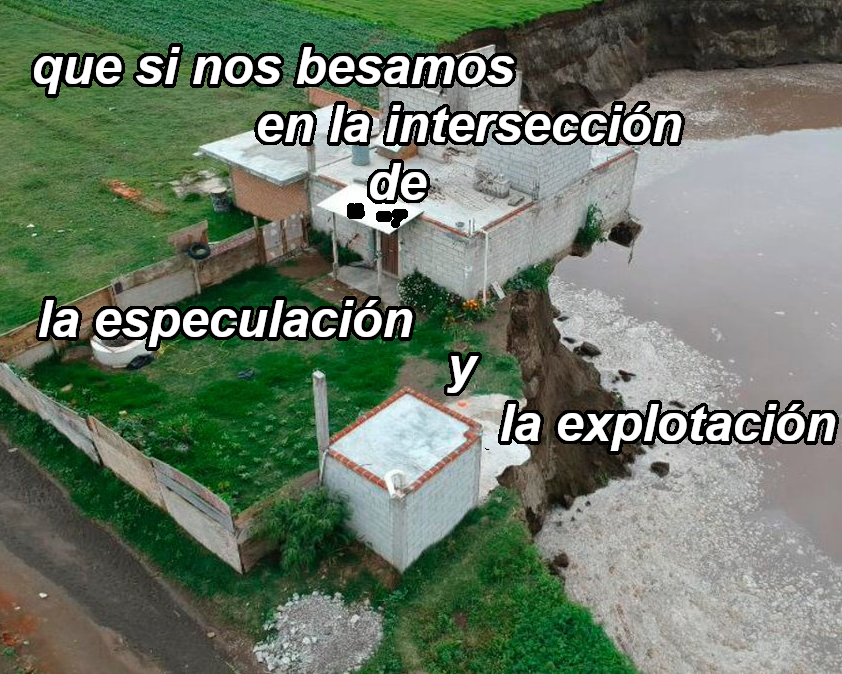
\includegraphics{images/8.png}

de juntar junquito seco para armarle

un nido al fuego y a pesar

de malos consejos de chabón

convertir brujamente la brasa en pájaro

paso ahora

la mano una llama de ebriedad y frío

a escuchar con tu amiga

las vibraciones nocturnales del río

``estoy inventando un ritual''

dice y en lo oscuro

nos corremos

del calorcito para crearlo nosotras

dulces corrientes de aire me ondulan

las piernas y de pronto sos vos

y de pronto es tu cariño

el cuero húmedo de este estuario

mareado ya no de escabio

entre la noche y su estrella

\url{https://64.media.tumblr.com/9adcf8a0bc7d845dea8692fd223cf373/8c4e7569dd6319bb-b9/s500x750/6cb02f9d832e346df3766a7ce2cf800238688be6.gifv}

\hypertarget{soreto-lamebola}{%
\chapter{soreto lamebola}\label{soreto-lamebola}}

exangüe pirulo cacofónico

no tragues mi tierra adulterándola

que es un corro de vida prometida

para párvulos corsos encendidos

estéril macumba ensangrentada

sacá ya tus manitas de la timba

mi grupa tiene piernas y acaricia

pedalero el suelo de tus ruinas

bostezo por tu culpa autocumplida

mi sueño de marimbas colchonetas

en mi coxis desde tarsos y a mi rifle

que encabezan la revuelta de la milpa

no tengo en nuestra espalda la carisma

de tus cómicos y estultos fantasmitas

me como nuestras uñas y mis tripas

son un fiasco para el verso de la yunga

que en la orilla de la mente se redunda

como un tero puntiagudo de sus puntas

\hypertarget{amor-de-hombre}{%
\chapter{amor de hombre}\label{amor-de-hombre}}

floreció el amor de hombre

que hay en casa es un poco linyera

aunque no le gusta

que le digan así

porque además de linyera es un amor

de hombre sensible

los flashes del día le queman las flores

llora y se resquebraja en las hojas

puede estar cinco días seguidos pasado

entre el fisureo y el autoboicot

preguntándose cuando está solo si no son

las circunstancias

las que le engualichan el cora

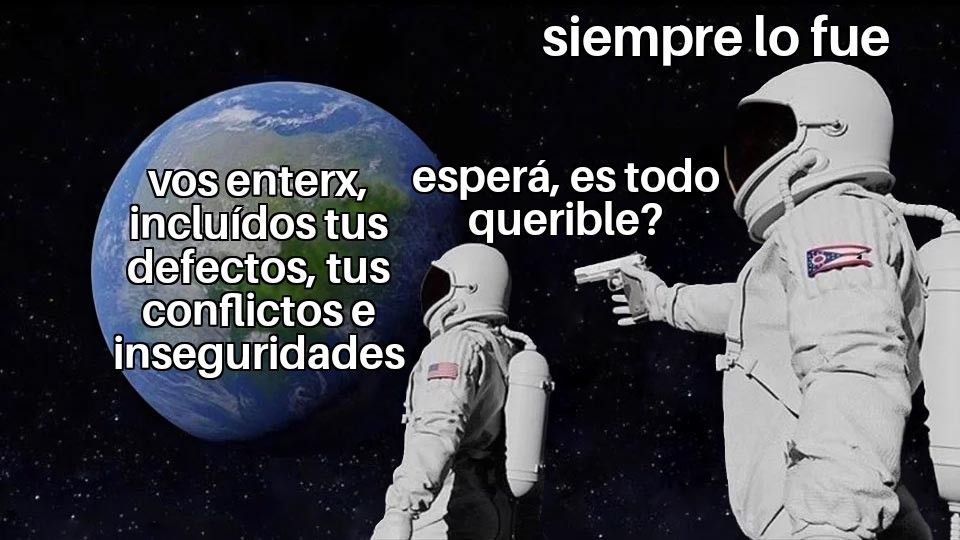
\includegraphics{images/9.png}

pero ah cuando venís vos

también vestido de violeta también

tierno y linyera

florece

y en toda su precariedad de primavera se sabe

perfectamente hermoso

hermosamente querible

\hypertarget{me-pierdo-en-un-bordoneo-porque-bordoneando}{%
\chapter{me pierdo en un bordoneo porque bordoneando}\label{me-pierdo-en-un-bordoneo-porque-bordoneando}}

me abandono de la palabra y quiero que seas

ahora de mi silencio una traba

o que en el diantre de la autoformación subjetiva constante de nuestras ánimas populares en este siglo eterno y flagelante

algo calle

de pronto

y pase o de paso al viento

me achaque de lo mío y junte la violencia

aprendida del mundo en mi carne

sea un desliz que por favor no te toque ni te muerda

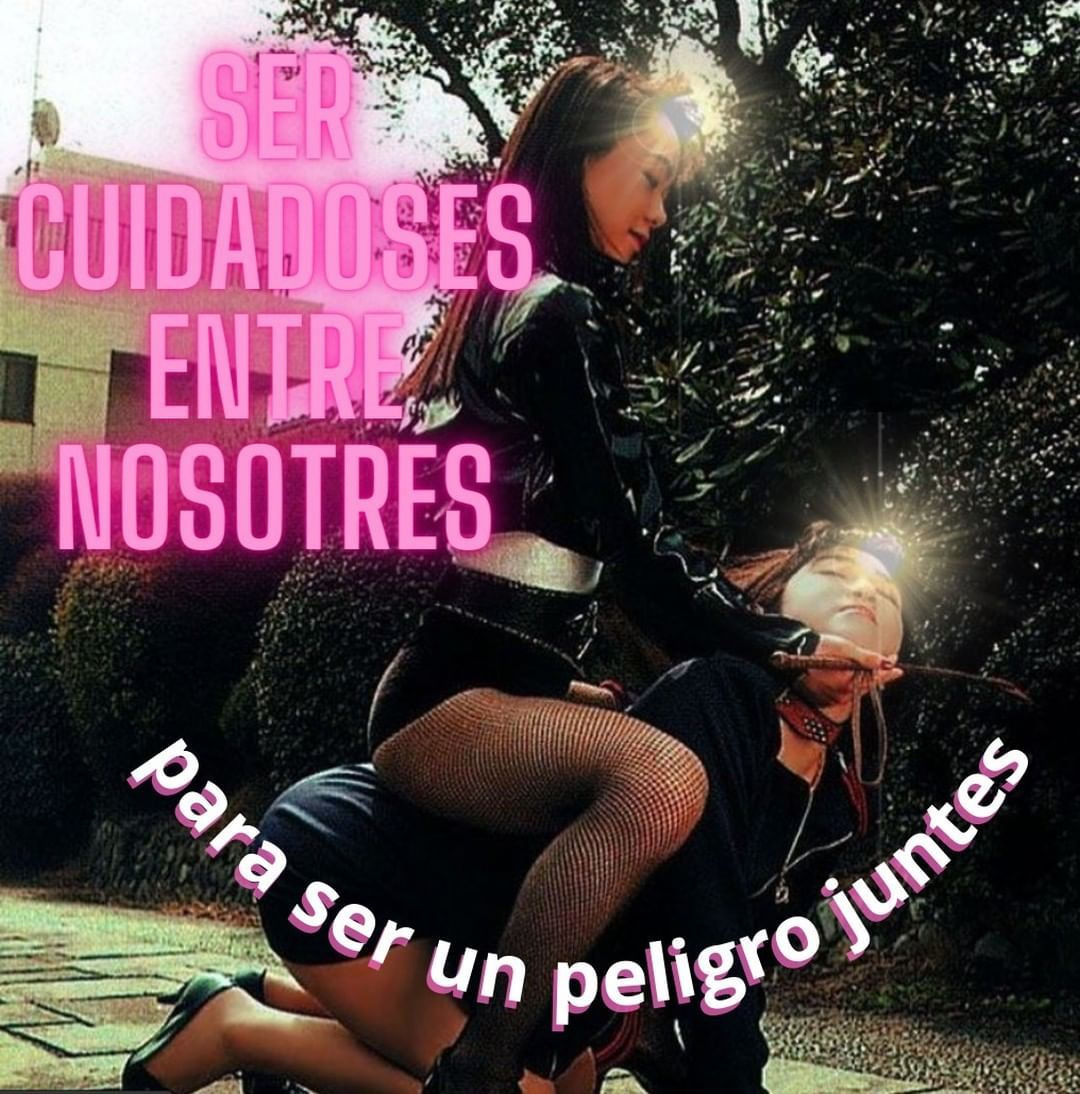
\includegraphics{images/10.png}

porque quiero también ser una rémora vertiginosa de papeles quemándose

en aceite usado o de ese orden malabar

medio curado por las nuevas narrativas metropampeanas con mueca cyborg

como si quisiera todo el tiempo saber cómo

se actualizan

las sensibilidades clasemedieras más perturbadas

me canso y me hundo puede ser

en las ruedas del calor que te convocan

por puro desperdicio por puro

año viejo recuperado en dos croquetas mal hechas de todas

las cosas

que amé y perdí

es que a veces

el vamoacharlarlo mejor se cancela y deja

espacio a otros fluidos discursivos

que toman tal vez la forma de un bardito o una mosca en el espacio

y decidamos no matarla decidamos

que lata con tal de sentir nuestros coras sobrevolando el enrosque

sonando con mayor o menor intensidad según su errancia

antes de que vuelvan finalmente monigotes

las bandurrias perdidas como un reflejo

casi nocturno de un mar árido quizá

o de esa lata de cerveza vacía que nos mira desde un charco en la vereda

a confundirse con nuestros sueños

sueños mochos exiliados del tiempo

pero que el beso de suelo y cielo todavía reclaman para sí

y devoran insecticidas las soledades cosechadas de tanta

calaña semiautoinflingida

que surcan modo cáscara las paredes y los campos

porque somos ese pasto y yo te quiero

tanto

que a nosotras van

mis horas jóvenes como fantasmas de una nuca que te sopla para no

asediar las introspectivas intocables ni enredar

de más las lenguas en el cuero

de este apocalipsing performado en el entonces qué

nos gotea y de ahí

de nuevo la mosca de un favor entumecido

donde ya no sé sabe quién le debe qué a quién

todo eso estremece y se cuece

en el sendero semiurbano que elegimos juntas

caminar pero sin saber nunca

bien adónde lleva

ni quién lo traza realmente tengo

en las líneas de tu mano la silueta de mi cuerpa mixturada

por la sangre celeste y la biografía periférica

por la historia de esta tierra que se nos cuela por todos los agujeros y las venas

esa es la única huella que sigo

y ojalá me pierda

\hypertarget{ponuxe9-tu-ansiedad-al-servicio-del-bien-comuxfan}{%
\chapter{poné tu ansiedad al servicio del bien común}\label{ponuxe9-tu-ansiedad-al-servicio-del-bien-comuxfan}}

ay amiga hay

cosas a veces más urgentes que someterse

siempre a las tiranías del estrés

por ejemplo podríamos

intentar sincronizar las ansiedades y a partir de ahí

una autogestión colectiva de la manija

que despeje no la precariedad

en general pero sí lo que no hablamos

y deje paso a roles un poco más

rotativos menos acelerados

para evitar con la mayor

ternura posible el x2 en las temporalidades

comunes que tenemos y lo sabés

que recuperar

o sucumbir

ya naturalizamos demasiadas de las forradas

que se nos impusieron en nuestra mediación social

en nuestro producto vivo

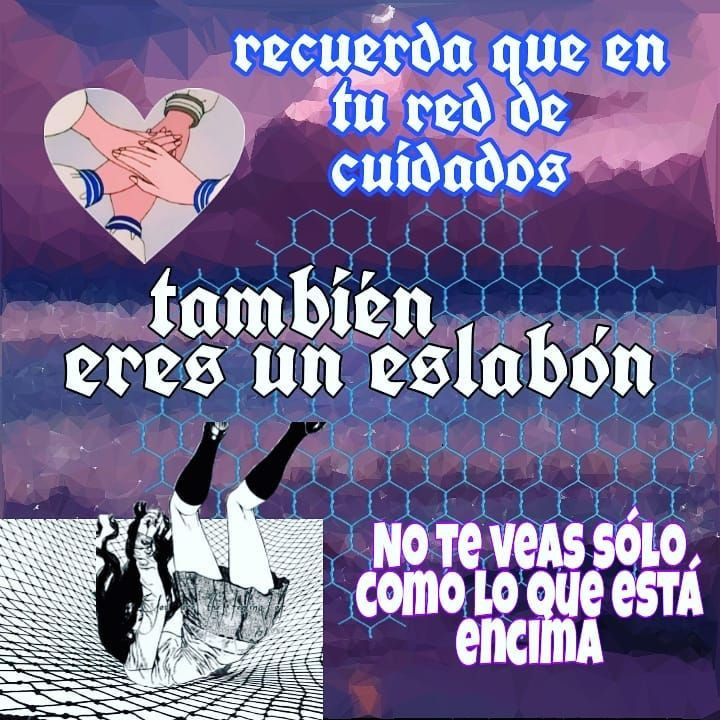
\includegraphics{images/11.png}

decí basta amiga basta

relajá un toque aunque delires

que no puedas

porque muchas cosas en la vida son cuestión

de perspectiva

y muchas otras lo son de expectativa

será que ahí es donde hay que reajustar y reagruparse

cosa de cuidarnos entre nosotras

para ser un peligro juntas

\hypertarget{formas-del-valor}{%
\chapter{formas del valor}\label{formas-del-valor}}

montarse sobre dos ruedas te

corta la bocha de una secuencia larga

el rodado mínimo hace de la perspectiva

un corcho o un ataúd pronunciado

para la visibilidad de las curvas

donde el relieve y lo que se corta

en la tarea holística de diagramar una ciudad

saben decir ``estas aves

están migrando sobre mí'' o ``mijael

rodríguez número 221 743-1982

perdió en esta esquina su billetera''

son las visiones que te hacés mientras

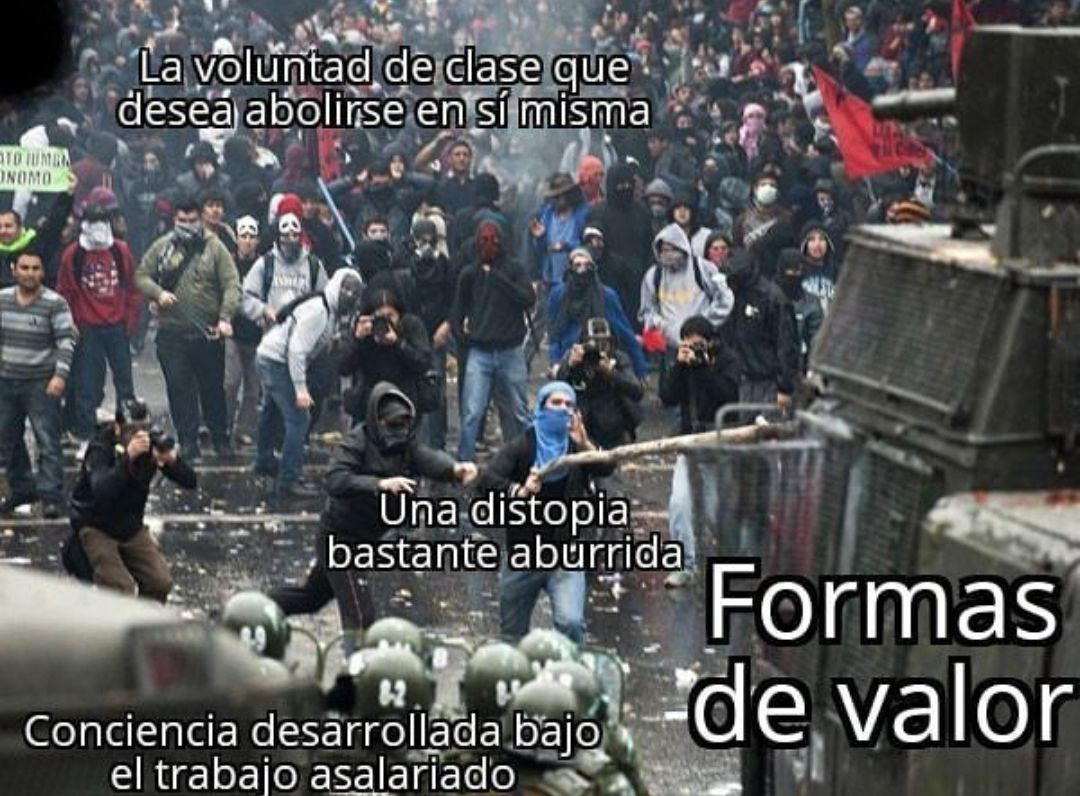
\includegraphics{images/12.png}

pedaleamos en la lluvia y a la carga

los perros vivos del trabajo precario

generando energía o liberando

plusvalor en la tracción de un paquete

que hay que entregar fresco

ya sea helado poesía u otros plásticos

en la carrera soltada de nuestros espantos

en las vías corridas de qué cadenas

de distribución y alarma porque viene

envenenada esta manzana de coltán

y tenemos internet cinco ge y un alfajor

de seitán gluten fri pero nuestras vidas

siguen más o menos igual veo el tendido

eléctrico marcar nuestro recorrido

mientras en la plaza alguien agita en la guitarra

canciones de misa: alaridos

que no claman ya más nada

mucho menos trascendencia -solamente

un desagüe de ilusión para las ranas

que encuentre mijael su billetera

\hypertarget{no-suxe9-si-es-el-quuxe9-o-este-cielo}{%
\chapter{no sé si es el qué o este cielo}\label{no-suxe9-si-es-el-quuxe9-o-este-cielo}}

\begin{verbatim}
_Estamos en una encrucijada de caminos que parten y caminos que vuelven._
Raúl González Tuñón
\end{verbatim}

para que bebamos la dulce fritura

del vendedor de punta lara

para que amemos santiago y managua

la paz y chiapas, pampas y cerros

los grises barquitos areneros

y la luz de las altas rompientes de la tarde

encendidas para los detectores de metales

y para los ladrones

y las placas en donde los yanarkas

tragan polillas nocturnas, escarabajos

y les niñes pochoclos del pochoclero

y bajo el sol y bajo los eucaliptos

entre ágiles malambos suenan

todas las cuerdas

placas, dije, las placas

continentales, platillos

del bajo caracas para el tambor

que es esa voz bajando

por el juncal alegre

tener un corazón ligero! vale decir

amar a todas las personas bellas

y una ética fiera, vale decir, andar

con fisuras alegres y dormir

en una sombra un ocaso cualquiera

y en otra sombra y en otra

y andar con suavidad y con desenvoltura

de fumador viajero

para que a cada paso un territorio

o una conmoción o una contrariedad

nos reconcilien con la vida pequeña

y su muerte pequeña

para que un día

nos queden

unos cuantos recuerdos, decir estuve

estuve en tal pasión, en tal retazo de sol

estuve, por ejemplo

en la feria de tilcara una mañana

con un pedazo de asado, una amistad tranquila

la mesa clara, las lagañas del perro, una conversación

y afuera, las tortilleras de la puna

chapoteando con los bombines en la nieve

para que bebamos la dulce fritura

del vendedor de punta lara

es necesario no asustarse de partir y volver

camaradas, de perderse en un bondi

y quedarse varadas

en una fundición de cielo

y montaña y playa y yunga y tierra

parda que anuncien los caminos

que se van y que vuelven

bajo el fin del armisticio al son

de esta vez quizá a nuestro favor

por un momento al menos grácil

grácil y breve

y nos olvidemos compañeras

no sólo de las olas

tiernas como eso, como olas

que acuerpamos calientes, somos

paladar de estas áureas

comillas de la noche

superpuestas en colpas tequeñas

bordemares, grasientas

muchedumbres y canciones, canciones

para que bebamos

la obscena fritura del vendedor de punta lara

\hypertarget{su-nombre-significa-cosechadora-de-almas}{%
\chapter{su nombre significa cosechadora de almas}\label{su-nombre-significa-cosechadora-de-almas}}

como en la noche un espanto

es su cuerpo entero parece

leche derramada

sobre los vidrios rotos camina

flácida o se difumina yo creo

me observa en lo oscuro

pero no con los ojos

hay algo en su cora

que me intuye

y que me ignora

\hypertarget{tkm-btw}{%
\chapter{tkm btw}\label{tkm-btw}}

\begin{verbatim}
_podríamos ser tan buenos, sino fuera por las circunstancias!_
s. zizek
\end{verbatim}

de pasta en pasta viven los yanquis pobres

dan penita ni bien verlos

en el cobertizo, en las paredes

hay un agujero negro que los traga

les imprime en la madera una señal bifronte

primero para el anca tibia y puritana

donde mi amigo les tatuó un lovecraft entumecido

por la marea de todos los océanos conquistados

en la otra faz un jimi hendrix con cadenas

industriales la cabeza

de águila imperial se pasa de rosca y babea

senil la gota gorda protestante

en pose onda san jorge lobotomizado


\includegraphics{images/13.png}

cositas

imaginaron una colina y vaya

que la levantaron sí

ahora tiene ese pico la cabeza medio torcida medio

carbonizada con la forma y los ojos de jeff bezzos

vuela en un cohete flácido hacia el vacío más cruel

y nuestro reptiliano favorito el que maneja

los mil feedlots algorítmicos de la mercancía

digital?

ay digo

no se le queman en ningún

ritual de sanación los bitcoins arrugados sus pasiones

maquínicas

la sangre fría tiene como todo

sus efectos colaterales

y al pobre hombre al más hondo

explorador de la humanidad que los padres fundadores

que los primerísimos pioneros jamás imaginaron

a los treintipico años

no se le para

y sin embargo todas tenemos sus pudores

nocturnos bien impresos en las manchas

de nuestras remeras

porque no somos acaso, de mañana

y de tarde imagen

y semejanza de estos ay tan tiránicos y modernos dioses nuestros?

dioses tristes podés decir

para el olimpo del proceso del valor

en tu sensibilidad y en la suya

y en la mía también habita un fondo de inversión

un conglomerado empresarial que

aparece

blurreado

pero bien que lo amamos

le dedicamos la fatiga y el logo

capitán amérika en cada niño del condado

mientras suena el aspaviento como un tanque sobre la escarcha

y recorre nuestros barros cantando épicas bélicas


\includegraphics{images/14.png}

con voz de gallo al ladrido de los perros

invisibles todavía pero epa

muy bien representados

casi como en un

cuadro realista se arden

en nuestras lenguas y cuerpas

entonces una pesadilla agria da vueltas al mundo con métrica vintage

quiere declamar su perigeo shitpostero con no sé qué

poesía del yo la lírica oxidental

como un modo de anunciar las profecías primordiales

pero cruzadas de hospicios y demonios todos

en la misma peli

moribunda de terrores liberales crezcan siempre

en tu pechito sideral

un dólar a la frente de cada animal pero también

de cada ánimo intersectado por la

circulación de capital ficticio unas croquetas

puestas en abismo

no digamos

fascismo o distopía

ni el candado

se abra oxidado en la reserva federal más netflixera

porque quién o cuántas van

a liberar el código de los astros

para la bajeza aspiracional que corre

como perro koi contra la corriente

periférica de la tasa depresiva de ganancia

si la colina de la capitol hill ahora termina

donde empieza mijos

su patria expandida de yerifs angustiados

en modulación barroca o de humo o de falopa

casi ozymandias de calores bajos

erosionándose fieramente con los vientos inclementes de la historia

un sol que nació

pobrecito hay que decirlo

algo idiota

y se reduce ahora de vuelta a su aldea y a la nuestra

se corta el chorro que da lástima

parda y culposa de que el mago blanco en su

blanca demencia nos deje de soñar

el alma súbita y el estrago

de su pico diamantino que horada los cueros nuestros

ni un imaginario fluviar sin enturbiar

ni un materialidad futura sin contaminar

que nos han dejado

para la pírrica hora de los pueblos

\hypertarget{un-himno-para-nuestra-junciuxf3n}{%
\chapter{un himno para nuestra junción}\label{un-himno-para-nuestra-junciuxf3n}}

si las profecías climatológicas que anuncian que para el sábado

estaremos libres ya de esta lluvia espuria

no erran como tienen por costumbre

a lo mejor

digo

podríamos ir al parque

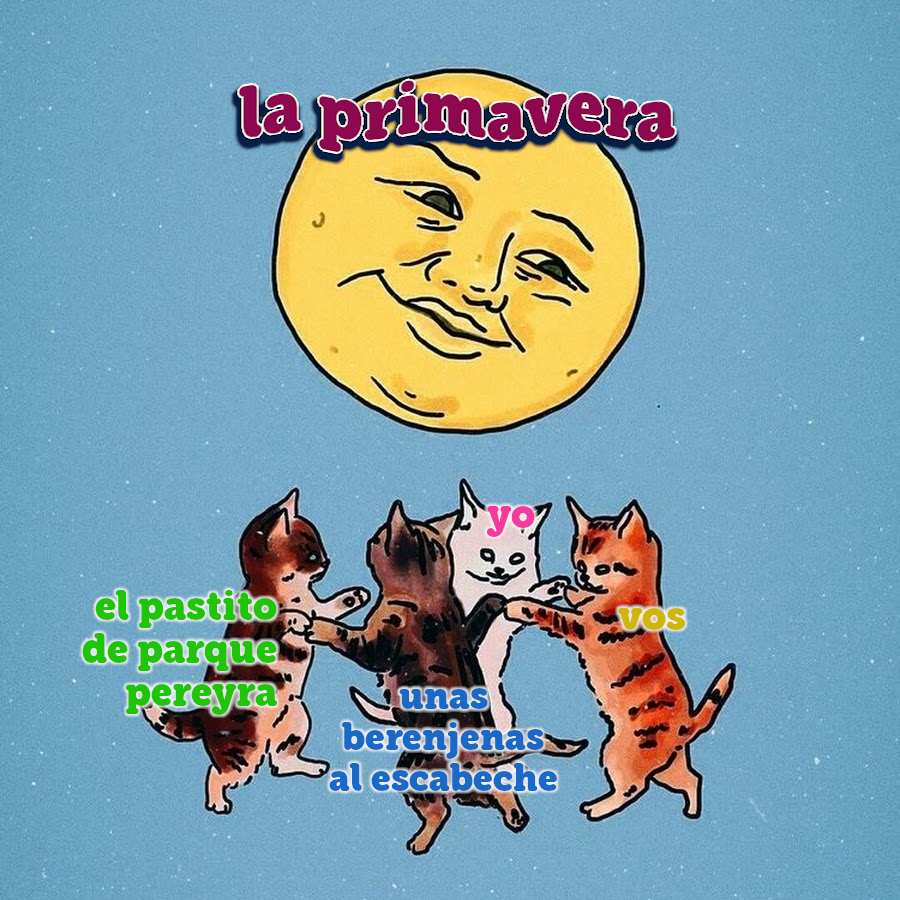
\includegraphics{images/15.png}

como supimos convenir a celebrar un aquelarre de invocación a la primavera

meta porro vino y lo que sea

atendiendo por otro lado el llamado de la naturaleza cíclica

porque somos fantasmas nunca ángeles y no sabemos

cuándo invocamos y cuándo estamos siendo invocadas

estas son nuestras presencias jóvenes que laten desde atrás y huelen las flores y se visten lindo o

trabajan cuando pueden la forma de su espalda

tengo también para mí el sonido de los pájaros como evocación

de los árboles altos que mueve el viento -y a los enamorados el pensamiento- pero también de una manera de la amistad

que paseando por las calles rosarinas me refería las características de la avifauna local

sonante a nuestros pasos

una de las aves en cuestión lo que hacía por ejemplo era ocupar los nidos de otras especies como gesto territorial expulsivo

otra era yo

tarareando barrio barrio

que tenés el alma inquieta de un gorrión sentimental

pasó ya el tiempo desde entonces pero de igual modo toda esa distancia todavía nos desune nos vuelve a unir y así sucesivamente

a nosotras nos separa otro bordoneo espectral

que galopa por los rieles pero también toda una extensión de pampa que se abisma por selváticos senderos

de bruma color nuestros vapores

con distinta gradación de luces sombras y espesores

para que floten libremente como soles

y viajen el uno hacia el otro sin apenas conocerse

nuestros ímpetus de gozosos corazones

porque llega la primavera y lo saben nuestras cuerpas

en ese tren las vestimos las disponemos

y en ese tono ajustamos lo mismo nuestras lenguas que dicen sí

nos veamos tengo ganas me pinta la idea qué planazo

porque el deseo es más de rodearse de pasto y de furor

florecido pero también

de pieles en roce incluso bocas que se juntan y se chupan

sutilmente en el chat y en el encuentro

presencial quién sabe

quisimos venir al parque y ver

árboles hongos

flashar romance en forma de amistad

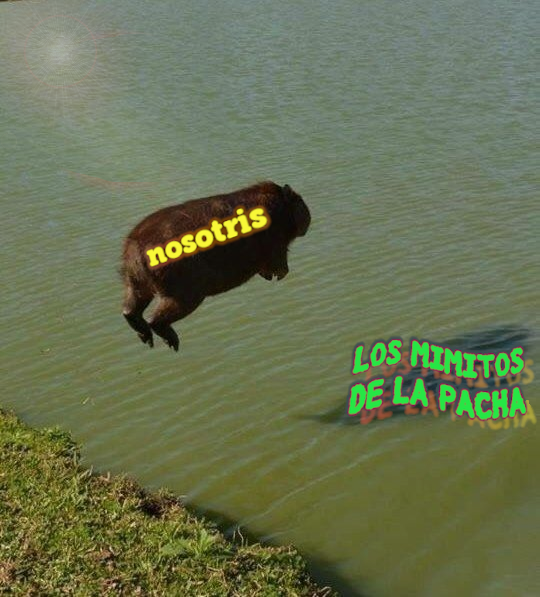
\includegraphics{images/16.png}

y conocer la armonía la dulce policronía de las tardes fabriqueras

desde la ventana empolvada

de un furgón muchacho mientras venimos

y entronamos en nuestras cabezas el decoro recíproco de maquinar

cómo me pongo linda para vos

si te prometí implícitamente cariño y fantasía

un alma brava a vos dispuesta

cómo vamos además a caer

en ese abismo de pasaje

a otras formas de escanciar lenguas y cuerpas

me decís

te quiero mucho por escuchar mis playlists

te digo

hice este meme para manijear nuestra juntada

aunque de tan candombe una me arruine

me corte de mandinga y me acuerdo de lo mío

porque ahora quiero

que veas mi casa una sirena que se enreda en estrellas de cemento sobre una ciudad cruzada

y florece para vos

sin aguantarse a que despeje

regida puramente por la pasión estacionaria a la fuerza de tu cara

performada en una selfi sacada exclusivamente entre nosotras

entonces los árboles los árboles

que arrancan a mosquearse a nuestra gira

pastito bragado de hormiguitas que somos

soñantes de marisma y distancia bien rompida

porque es eso el parque se presta a una

proxemia pagana que sabemos construir

con sudor y sin pudor

para apoyar el mantel con parsimonia fornida en el agujero del arenal

cosa de hacer del espacio una fuga temporal merecida por nuestro agite

y nos arrimemos

a compartir el vino el calorsito estas pulsiones

de sábado hermoso

armado

meramente

a las señas varias del amor súbito en mansedumbre

mientras con los ojos cholos contemplamos la caída

brusca de la civilización occidental pero también

de sus tipologías del afecto

embrutecidas en la gestión mercantil de los deseos

y ruedan en nuestras manos de mediodía la belleza que nos junta

y ese polen que exhalan sin vergüenza las veredas y los bosques

como cantando un poema lírico sobre la importancia

de expropiar espacios verdes

a distancia proletaria

entre metrópolis terribles

donde mechar una lona y hacer el fuego que nuestros coras piden con ramitas y hojas secas

los celulares en silencio sólo las corrientes de aire dirigiendo

la música de la noche esa estrella borracha

que al calor de la luna nos vuelve extrañas de hermosura

pero grandes y posibles

porque mientras la carne se macera en la brasa que nos abriga algo somos

de utopía y de asedio y de incandescencia y nunca unas

manos al humo

solitarias no

abolimos la soledad y también la felicidad

más al fondo entonces las cumbias retumban como un eco de guaracha

un grito de guerra para la necesidad de una danza taimada que ponga en juego

la necesidad física

abreve los placeres

al cauce del viento y de nuevo a los pájaros

que no por chirria son capaces de sonar al compás de las vestiduras humanas

sus rituales nocturnos concedidos al brebaje espirituoso

materia afín que nos arrastra la una tan cerca

tan cerca de la otra

son orejas de la precariedad y el aislamiento nuestros pulsos

pero que vienen desde antes se diría acaso

los tiempos de la colonia y el trabajo

rastro que habita a todo esto en la corteza milenaria de nuestros cueros y ambientes sobre los que quizá

ahora nos recostamos suaves ya cediendo ya sedientas

ya no de alcohol sino de estos jugos

que nos regala el nuevo clima

a las anatomías jóvenes no

sino a las corazonas que cancelamos lo más gris de este futuro

y marcamos nuestro pecho

con sangre arrebatada a los flujos

incesantes del valor para preparar así con todas

las armas de la querencia

nuestro gesto barroco

de inventarnos una vida en medio de la muerte

\hypertarget{psico-fracking-urbano-de-tus-fantasuxedas-cyberpunk}{%
\chapter{psico-fracking urbano de tus fantasías cyberpunk}\label{psico-fracking-urbano-de-tus-fantasuxedas-cyberpunk}}

en la puerta tapiada

de las ruinas de un cyber

dos carteles de papel:

arriba espert 2021 la

senilidad discursiva

del capitalismo tardío te sonríe

calva y pidiéndote que lo votes

te baja el pulgar

abajo en tipografía de

recital tecno o peli futurista

CRISTO VIENE PRONTO

¿estás preparado? el flash

evangelista cierra

con 2 pedro 3:10-11

\begin{verbatim}
“Pero el día del Señor vendrá como ladrón en la noche;  en el cual los cielos arrasarán con grande estruendo, y los cinco elementos del mundo nuestro arderán y serán deshechos, y la tierra y las obras que en ella hay serán  quemadas enteras, con suplicio de la humanidad y de todas las razas vivientes”. 
\end{verbatim}

  \bibliography{book.bib,packages.bib}

\end{document}
